\chapter{Herramientas de evaluación de algoritmos}

\section{Introducción}
La solución de software propuesta, es un conjunto de bibliotecas desarrolladas en lenguaje de programación C++ orientado a objetos. Este grupo de bibliotecas de clases posibilitan, por una parte, construir una simple aplicación cliente, que incorpora los algoritmos de visión de computador que se quieren verificar, y por otra parte, evaluar resultados logrados con el cliente proporcionado por este sistema (u otro independiente). Comparando posteriormente, el resultado con las imágenes de referencias, suministrada por el conjunto de datos que esta bajo evaluación. El software proporciona las interfaces necesarias, que simplifican la creación de instancias, de los algoritmos incluidos en el sistema de software. Facilita también, la incorporación de nuevos algoritmos, encapsulando las bibliotecas (de estos algoritmos) en una clase que contiene las operaciones predeterminadas, reconocidas por el sistema de software. 

Otro aspecto importante de esta solución de software, constituye la herramienta de evaluación de desempeño. Ésta fue proyectada, desde un principio, como un cliente que recibe de entrada un conjunto de imágenes procesadas, y otro conjunto de imágenes de referencia (\textit{ground-truth}). La salida es un resumen de desempeño, producto de la comparación de cada imagen. Este diseño, es independiente de la plataforma sobre el cual se ejecuta el algoritmo medido. La evaluación se realiza sobre las imágenes resultantes, previamente procesadas por los algoritmos que se intentan medir. Esta herramienta de software, incluye la serie de métricas más comunes utilizadas en segmentación de imágenes, y un par de métricas relacionadas con la medición de percepción (similaridad estructural o métrica D-Score). El producto final es un archivo de texto, que contiene los resultados obtenidos para cada imagen y un valor acumulado total que informa el desempeño global del algoritmo logrado en toda la secuencia.


\begin{figure}[h!]
\centering
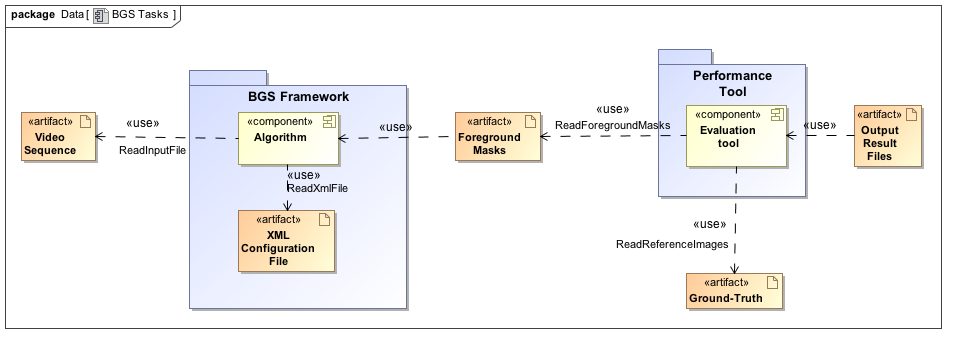
\includegraphics[scale=0.5]{img/BGS_Tasks}
\caption[Diagrama de componentes]{Diagrama de operación de los componentes de software.}
\label{fig:bgs_tasks}
\end{figure}



\section{Arquitectura de Software}

La arquitectura de software está basada en módulos. Cada módulo es una unidad independiente de software, basado en programación orientada a objetos. Facilita un conjunto de clases en C++, para ser utilizadas por los programas clientes, en los distinto niveles que ha sido estructurado de la arquitectura de este software. Los distintos módulos hacen uso de las bibliotecas de otros módulos para utilizar las facilidades que proporcionan cada uno de ellos.  

\begin{figure}[h!]
\centering
%\fbox{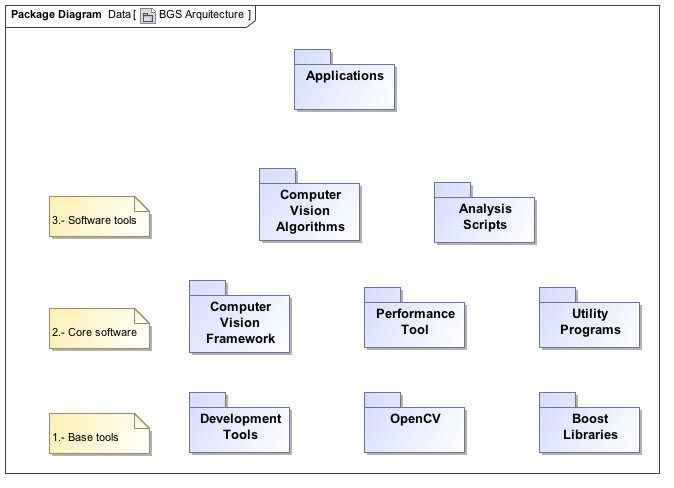
\includegraphics[scale=0.8]{img/BGS_Arquitecture}}
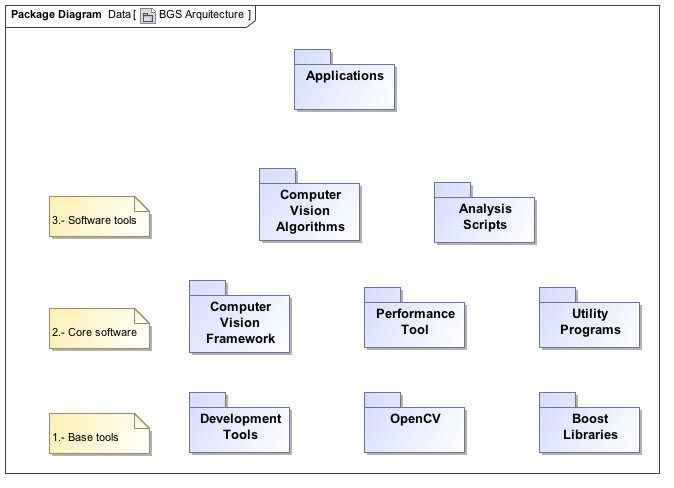
\includegraphics[scale=0.7]{img/BGS_Arquitecture}
\caption[Arquitectura modular de software]{Diagrama de la arquitectura de software propuesta.}
\label{fig:arq_software}
\end{figure}
 

\subsection{Herramientas Base}

La primera parte esta constituido principalmente, por las herramientas de desarrollo utilizados, como el compilador de C++, el repositorio de software donde se mantiene el control de versiones de los módulos. Las bibliotecas de OpenCV y Boost.

\subsubsection{Herramientas de desarrollo}
El desarrollo de los diferentes módulos de este software ha sido realizado en una distribución Linux, \textit{Ubuntu} 12.04 LTS precise. Ubuntu es un sistema operativo Linux, basado en Debian, que incluye todas las herramientas necesarias para hacer la implementación de los paquetes de software de esta solución. A continuación, se hace una breve descripción de los diferentes productos utilizados.

\begin{itemize}
\item \textbf{Compilador} GNU GCC versión 4.6
\item \textbf{CMake} es un grupo de herramientas, \textit{open source} independiente del sistema operativo, diseñado para construir, validar paquetes de software. Se ha usado principalmente para generar los archivos \textit{Makefile} nativos al sistema operativo Ubuntu. La utilidad de CMake, radica principalmente, en la independencia de la plataforma sobre la cual se está desarrollando. En caso de ser necesario, los módulos de software también pueden ser compilados y ejecutados en otros ambientes (MAC OS X, otros ``distros'' de Linux, o Windows).
\item \textbf{Servidor de repositorios \textit{GitHub}}, para llevar el control de cambios de versión de los distintos módulos. Este servicio de repositorio público, se basa en \textit{GIT} un sistema de control de versiones distribuidos. Las principales características, entre varias otras más, es un sistema de control de los datos, almacena el estado de un proyecto a nivel de directorios y archivos. Crea un registro completo (\textit{snapshot}) del repositorio que esta siendo almacenado, esto facilita las tareas de recuperación, creación de ramas de desarrollo (\textit{branch}) y unión (\textit{merge}) de diferentes versiones de un módulo. El proyecto completo puede ser localizado en el siguiente URL: \textit{https://github.com/jorgesep/BGS}. 
\end{itemize}


\subsubsection{Biblioteca OpenCV}
OpenCV \cite{opencv} (\textit{Open Source Computer Vision Library}) es una biblioteca que contiene una gran cantidad de algoritmos muy utilizados en visión por computador. La API (\textit{Application Programming Interface}) de OpenCV comprende una serie de módulos, que abarcan varios de los aspectos que se requieren para construir una aplicación en visión por computador. El módulo principal, define las estructuras básicas sobre la cual se desarrollan todas las aplicaciones, incluido los módulos de software construidos en este proyecto de tesis. Establece un arreglo, denominado \textit{Mat}, de varias dimensiones que permite contener en forma nativa,  la estructura de una imagen sobre la cual se pueden hacer todas las operaciones matriciales básicas, necesarias en visión por computador para manipular imágenes. Incluye también, un modulo de procesamiento de imágenes (filtros lineales y no-lineales, transformación geométrica de imágenes, conversión de espacio de colores, histogramas, entre otros). Un módulo de análisis de videos, que contiene varios algoritmos, entre ellos el algoritmo (\textit{Background Subtraction}) original de  \textit{Zivkovic y Heidjen} \cite{zivkovic_efficient_2006} evaluado en este trabajo.  Se agregan además, algoritmos de calibración, detectores de características, detección de objetos, una interfaz (\textit{gui}) para la captura de imágenes de video, \textit{codecs} de imágenes. También incluye un módulo para trabajar con GPU.


\begin{figure}[h!]
\centering
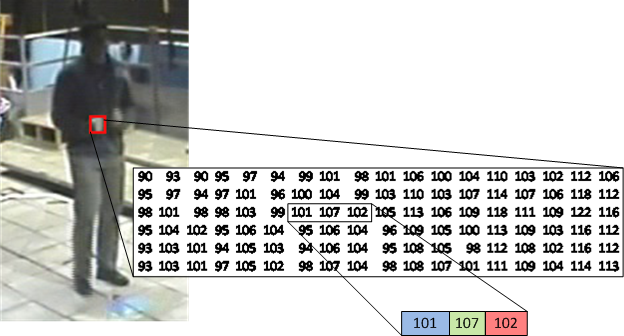
\includegraphics[scale=0.7]{img/Opencv_mat}
\caption[OpenCV arreglo Mat ]{Descripción del arreglo básico MAT de OpenCV}
\label{fig:mat}
\end{figure}


La estructura de datos \textit{Mat}, es una clase C++ de n-dimensiones, constituida en dos partes. Tiene un encabezado de la matriz de datos, que contiene información del tamaño de la matriz, el método utilizado para almacenar la matriz, la dirección de memoria donde se encuentra localizada la matriz de datos, entre otro tipo de información. Mantiene también, un puntero de la zona de memoria donde se encuentra la matriz de píxeles, y su dimensionalidad depende del método empleado para almacenar los datos. El encabezado de la matriz es constante, pero el tamaño de la matriz varia dependiendo del tipo de imagen que esta siendo manipulada. La figura \ref{fig:mat} es un ejemplo de esta matriz, la zona demarcada por el rectángulo en rojo es una zona de interés que se desea estudiar. La zona es una matriz de números manejada por la matriz \textit{Mat}, en el caso de una imagen definida en el espacio RGB, se almacenan los valores de cada píxel, en forma contigua, en el orden: blue, green, y red.\\


\begin{lstlisting}
Mat A, C;                   // creates just the header parts
A = imread("File.jpg" , CV_LOAD_IMAGE_COLOR); // allocate matrix
Mat B(A);                   // Use the copy constructor
C = A;    
\end{lstlisting}

\subsubsection{Biblioteca Boost}
Boost \cite{boost} se ha usado principalmente para, evitar el problema que se encuentra al manipular archivos, operar con \textit{strings} de caracteres en C++. \textit{Boost} contiene varias bibliotecas utilitarias, y en este proyecto se han usado especialmente las que permiten manejar expresiones regulares, búsqueda de caracteres en una linea de \textit{strings}, reemplazo de caracteres, manipulación de archivos: $boost::filesystem$, $boost::system$, $boost::program_options$, $boost::reg_exp$.


\subsection{Descripción de sistemas de software}
La segunda capa del sistema de software implementado, está compuesto por dos módulos principales e independientes. El primero corresponde a un \textit{Framework} de software que incorpora los algoritmos que requieren ser evaluados. El segundo módulos es una programa que efectúa evaluación de desempeño de los resultados obtenidos por los algoritmos. 
